\section{Experiments}
\label{sec:exp}

\subsection{Setup}
\label{sec:setup}

\paragraph{Students, teacher, and data mixtures.}
Students are frozen \texttt{Qwen3} LLMs~\citep{yang2025qwen3} ($0.6$B, $1.7$B
default, $8$B), supervised by \texttt{Qwen3-VL-8B-Instruct}~\citep{bai2025qwen3vl}
($27$-layer, $0.41$B ViT; inference-only in \modelname-Tower). We evaluate three
mixtures (Sec.~\ref{sec:supp_data}):
(1) \emph{base} ($21$k train / $2{,}408$ val): short-answer visual reasoning
(${\sim}70\%$ MC, $30\%$ numeric/short text);
(2) \emph{+open} ($28$k train / $3{,}388$ val): adds $8{,}334$ open-ended
items ($6{,}500$ doc/chart~\citep{mathew2021docvqa}, $1{,}834$
GQA~\citep{hudson2019gqa}) and $2{,}101$ plane-geometry items; and
(3) \emph{debiased} ($44$k: $39{,}949$ train / $4{,}441$ val): removes all
SHA1 and $64$-bit dHash (Hamming ${\le}2$) matches against all $7{,}552$
benchmark images, enforces image-disjoint splits, and balances A/B/C/D
($1{:}1{:}1{:}1$) and Yes/No ($1{:}1$) labels.

\paragraph{Benchmarks and protocols.}
We evaluate zero-shot accuracy on MMStar~\citep{chen2024mmstar} ($1{,}500$),
HallusionBench~\citep{guan2024hallusionbench} ($951$), MathVista
testmini~\citep{lu2024mathvista} ($1{,}000$), ChartQA~\citep{masry2022chartqa}
($2{,}500$), OCRBench~\citep{liu2023ocrbench} ($1{,}000$), and Geometry3K
test~\citep{lu2021geometry3k} ($601$), plus pure-text GSM8K~\citep{cobbe2021gsm8k}
and ARC-Challenge~\citep{clark2018arc}. Multiple-choice and yes/no items use
candidate-string likelihood across all main tables, while open-ended items use
unified greedy decoding (no per-benchmark token bans) with official relaxed
metrics; full free-form audits (\texttt{--force-gen}) appear in
Tab.~\ref{tab:supp_fgen}. We report \emph{MC2} (MMStar, HallusionBench),
\emph{Core3} (+MathVista), and \emph{Avg6} (average across all six evaluation tasks).

\paragraph{Baselines and implementation.}
All baselines share the frozen $1.7$B backbone, data, $392{\times}392$
resolution, and step budget:
(1) \emph{External tower}: \emph{LLaVA-Proj}~\citep{liu2024improved},
\emph{FastV}~\citep{chen2024fastv} (top-$32$), \emph{Spatial-Pool}
($32$-token spatial pooling~\citep{cha2024honeybee}),
\emph{ROSE}~\citep{rose2025}, and \emph{Hinton-KD}~\citep{hinton2015distilling} /
\emph{RKD}~\citep{park2019rkd};
(2) \emph{Encoder-free}: \emph{Patch-Merger Only} ($K{=}0$),
\emph{VoRA-style LoRA}~\citep{vora2025} ($r{=}16$, $K{=}4$), and
\emph{EVE-style Copy}~\citep{diao2024eve} ($K{=}4$, $201$M) atop the same
zero-deep-token SAVM interface;
(3) \emph{On-policy KD}: \emph{GKD}~\citep{agarwal2024gkd},
\emph{MiniLLM}~\citep{gu2024minillm}, and \emph{SeqKD}~\citep{kim2016sequence}.
Rotations use $b{=}64$, $d_q{=}256$, and layers $\{0,4,8,12,16,20,24\}$
($0.6$B/$1.7$B) or $\{0,5,10,15,20,25,30\}$ ($8$B). Reference $21$k/$28$k runs
use unbounded rotations with \texttt{hyb} ($6{,}000$/$2{,}500$/$3{,}000$/$500$
steps), whereas $44$k uses \texttt{qcond}+\texttt{direct\_hyb}
($\tau_{\mathrm{rot}}{=}0.12$; $2{,}400{+800}$/$2{,}200$/$1{,}200$/$600$ steps;
Tab.~\ref{tab:supp_hparams}). All $44$k runs use cross-entropy initialisation
(\texttt{ce}), while $21$k offline baselines also evaluate teacher alignment
(\texttt{rel}: $+0.5\mathcal{L}_{\mathrm{KD}}{+}0.1\mathcal{L}_{\mathrm{rel}}$,
Sec.~\ref{sec:supp_data}).

\subsection{Main Results}
\label{sec:main}

\begin{table*}[t]
\centering
\caption{\textbf{Main comparison across external baselines and \modelname{} variants}
($1.7$B frozen student, plus $0.6$B tower-free; single runs use $s{=}0$, with
$3$-seed means in Tab.~\ref{tab:supp_scale}). Comparisons are within-mixture
($21$k \emph{base} vs.\ $28$k \emph{+open}); detailed OPD objective ablations
(\texttt{GKD}, \texttt{MiniLLM}, \texttt{SeqKD}) appear in Tab.~\ref{tab:opd}.
``Tok.'' is deep visual token count; ``FLOPs'' is relative prefill compute at
$4{,}096$ patches ($1.00{\times}{=}9.85$ TFLOPs). Best per block in \textbf{bold},
second \underline{underlined}.}
\label{tab:main}
\small
\setlength{\tabcolsep}{3.8pt}
\resizebox{\textwidth}{!}{%
\begin{tabular}{@{}lcccc ccccc c@{}}
\toprule
Method & Mix & Tower & Tok. & FLOPs$\downarrow$ & MMStar$\uparrow$ & Hallu.$\uparrow$ & MathV.$\uparrow$ & MC2$\uparrow$ & Core3$\uparrow$ & Avg6$\uparrow$ \\
\midrule
{\color{gray}Teacher (Qwen3-VL-8B-Instruct, 8B)} & {\color{gray}---} & {\color{gray}0.4B ViT} & {\color{gray}all} & {\color{gray}$2.25\times$} & {\color{gray}65.80} & {\color{gray}72.45} & {\color{gray}63.20} & {\color{gray}69.13} & {\color{gray}67.15} & {\color{gray}59.03} \\
\midrule
\multicolumn{11}{@{}l}{\textit{With External Vision Tower (0.41B ViT, $21$k Base Mixture, $s{=}0$)}} \\
LLaVA-Proj~\citep{liu2024improved} (Full Tokens)        & $21$k & 0.4B ViT & all & $1.00\times$ & \underline{29.60} & 53.10 & \textbf{24.90} & \underline{41.35} & \textbf{35.87} & \textbf{21.02} \\
ROSE~\citep{rose2025} (Single-Freq Rotation, CE)        & $21$k & 0.4B ViT & \textbf{0} & \textbf{0.69$\times$} & 25.60 & \underline{54.36} & 19.70 & 39.98 & 33.22 & 17.14 \\
Hinton-KD~\citep{hinton2015distilling} (Off-Policy KL)  & $21$k & 0.4B ViT & \textbf{0} & \textbf{0.69$\times$} & 26.00 & 49.95 & 18.90 & 37.97 & 31.62 & 16.43 \\
RKD~\citep{park2019rkd} (Relational Feature KD)         & $21$k & 0.4B ViT & \textbf{0} & \textbf{0.69$\times$} & 26.13 & 51.31 & 19.20 & 38.72 & 32.22 & 16.70 \\
\textbf{\modelname-Tower (\texttt{mf}, CE, Ours)}       & $21$k & 0.4B ViT & \textbf{0} & \textbf{0.69$\times$} & 27.73 & 53.73 & \underline{20.60} & 40.73 & 34.02 & 17.67 \\
\textbf{\modelname-Tower (\texttt{hyb}, CE, Ours)}      & $21$k & 0.4B ViT & \textbf{0} & \textbf{0.69$\times$} & \textbf{30.60} & \textbf{58.15} & 18.50 & \textbf{44.37} & \underline{35.75} & \underline{18.36} \\
\midrule
\multicolumn{11}{@{}l}{\textit{With External Vision Tower (0.41B ViT, $28$k +Open Mixture, $s{=}0$)}} \\
LLaVA-Proj~\citep{liu2024improved} (Full Tokens)        & $28$k & 0.4B ViT & all & $1.00\times$ & \textbf{29.27} & 54.15 & \underline{25.00} & 41.71 & \textbf{36.14} & \underline{20.89} \\
FastV~\citep{chen2024fastv} (Top-$32$ Visual Tokens)    & $28$k & 0.4B ViT & 32  & $0.72\times$ & 28.53 & 49.74 & 24.90 & 39.14 & 34.39 & 19.43 \\
Spatial-Pool~\citep{cha2024honeybee} ($32$ Pooled Tokens) & $28$k & 0.4B ViT & 32  & $0.72\times$ & \underline{29.13} & 53.10 & \textbf{25.80} & 41.12 & \underline{36.01} & \textbf{21.06} \\
\textbf{\modelname-Tower (\texttt{hyb}, CE, Ours)}      & $28$k & 0.4B ViT & \textbf{0} & \textbf{0.69$\times$} & 28.27 & \underline{56.05} & 19.60 & \textbf{42.16} & 34.64 & 18.16 \\
\textbf{\modelname-Tower (\texttt{mf}+VL-OPD, Ours)}    & $28$k & 0.4B ViT & \textbf{0} & \textbf{0.69$\times$} & 26.80 & \textbf{57.41} & 23.50 & \underline{42.11} & 35.90 & 18.50 \\
\midrule
\multicolumn{11}{@{}l}{\textit{Encoder-Free Architecture (No Vision Tower, Offline, $s{=}0$)}} \\
Patch-Merger Only ($K{=}0$, \texttt{rel} init)          & $21$k & --- & \textbf{0} & \textbf{0.03$\times$} & 24.00 & 47.84 & \textbf{21.60} & 35.92 & 31.15 & 15.81 \\
EVE-style Copy~\citep{diao2024eve} ($K{=}4$, $201$M, \texttt{rel} init) & $21$k & --- & \textbf{0} & \underline{0.26$\times$} & 24.33 & 53.31 & 18.60 & 38.82 & 32.08 & 16.80 \\
Static Cayley Rotation (\texttt{rot} $K{=}4$, $2.3$M, \texttt{rel} init) & $21$k & --- & \textbf{0} & \underline{0.26$\times$} & 25.20 & \textbf{56.26} & \underline{20.20} & 40.73 & \textbf{33.89} & \underline{17.55} \\
VoRA-style LoRA~\citep{vora2025} ($K{=}4$ + \texttt{mf}, \texttt{ce} init) & $21$k & --- & \textbf{0} & \underline{0.26$\times$} & 23.73 & 49.95 & 18.50 & 36.84 & 30.73 & 15.82 \\
\textbf{\modelname-Free (\texttt{rots} $K{=}4$ + \texttt{mf}, \texttt{ce}, Ours)} & $21$k & --- & \textbf{0} & \underline{0.26$\times$} & \underline{27.33} & \underline{55.31} & 18.00 & \textbf{41.32} & 33.55 & 17.33 \\
\textbf{\modelname-Free (\texttt{rots} $K{=}4$ + \texttt{hyb}, \texttt{ce}, Ours)} & $28$k & --- & \textbf{0} & \underline{0.26$\times$} & \textbf{27.60} & 54.57 & 19.10 & \underline{41.09} & \underline{33.76} & \textbf{17.58} \\
\midrule
\multicolumn{11}{@{}l}{\textit{Encoder-Free + VL-OPD (No Vision Tower, $s{=}0$; Sequence-Objective Baselines in Tab.~\ref{tab:opd})}} \\
\textbf{\modelname-Free + VL-OPD ($1.7$B, +Open Mix, $s{=}0$, Ours)} & $28$k & --- & \textbf{0} & \underline{0.26$\times$} & 26.33 & 54.36 & 18.00 & 40.35 & 32.90 & 17.21 \\
\textbf{\modelname-Free + VL-OPD ($1.7$B, Base Mix, $s{=}0$, Ours)}  & $21$k & --- & \textbf{0} & \underline{0.26$\times$} & \textbf{27.93} & \underline{56.99} & \textbf{19.80} & \underline{42.46} & \textbf{34.91} & \underline{18.02} \\
\textbf{\modelname-Free + VL-OPD ($0.6$B, +Open Mix, $s{=}0$, Ours)} & $28$k & --- & \textbf{0} & \textbf{0.11$\times$} & \underline{27.53} & \textbf{57.83} & \underline{18.60} & \textbf{42.68} & \underline{34.66} & \textbf{18.05} \\
\bottomrule
\end{tabular}}
\end{table*}

Tab.~\ref{tab:main} (visualized in Fig.~\ref{fig:supp_mainres}) establishes four
conclusions under matched-data comparisons:
\emph{(i) Perception and anti-hallucination without visual tokens:} on $21$k
\emph{base} ($s{=}0$), \modelname-Tower (\texttt{hyb}) achieves $30.60\%$ MMStar
and $58.15\%$ HallusionBench ($44.37\%$ MC2, $+3.02$ over LLaVA-Proj) while
matching $99.7\%$ of its Core3 ($35.75\%$ vs.\ $35.87\%$) at text-only sequence
length $T$.
\emph{(ii) Diagram reasoning with grounded accuracy:} on $28$k \emph{+open}
($s{=}0$), \modelname-Tower (\texttt{mf}+VL-OPD) attains $23.50\%$ MathVista
and $35.90\%$ Core3 ($99.3\%$ of LLaVA-Proj, $+3.26$ HallusionBench).
\emph{(iii) Tower-free parity at one-quarter compute:} \modelname-Free{}
(\texttt{rots} $K{=}4$+\texttt{mf}) reaches $41.32\%$ MC2 on $21$k \emph{base}
(vs.\ $36.84\%$ VoRA-style LoRA), and VL-OPD lifts \modelname-Free{} (\texttt{hyb})
to $42.46\%$ MC2 and $34.91\%$ Core3 ($97.3\%$ of LLaVA-Proj) with $74.2\%$
fewer FLOPs.
\emph{(iv) Single-factor tier gains:} holding the deep tier at \texttt{mf},
\texttt{rots} beats rank-$16$ LoRA by $+4.48$ MC2 with $36\%$ fewer parameters
($2.40$M vs.\ $3.74$M); holding the encoder fixed, \texttt{mf} and \texttt{hyb}
beat single-frequency ROSE by $+0.75$ and $+4.39$ MC2 ($40.73\%$ and $44.37\%$
vs.\ $39.98\%$ on MC2).

\subsection{Scaling Across Student Sizes and Seeds}
\label{sec:scaling}

Across $0.6$B, $1.7$B, and $8$B students and three-seed runs ($s\in\{0,1,2\}$
on $28$k \emph{+open}; full numbers in Tab.~\ref{tab:supp_scale}), a $0.6$B
tower-free model already reaches $42.68\%$ MC2 at $s{=}0$
($41.52\%{\pm}1.39\%$ over three seeds), matching $1.7$B perception. Across
three $1.7$B seeds, VL-OPD lifts \modelname-Free{} from $40.36\%$ to $41.11\%$
MC2 and $33.24\%$ to $33.79\%$ Core3. Scaling to $8$B yields no further gain
($39.91\%$--$40.90\%$ MC2), indicating that the fixed-width frozen adapter
bandwidth ($d_q{=}256$, $K{=}4$)---rather than LLM capacity---sets the ceiling,
making compact $0.6$B deployment ($0.11{\times}$ FLOPs) particularly effective.

\begin{figure*}[t]
\centering
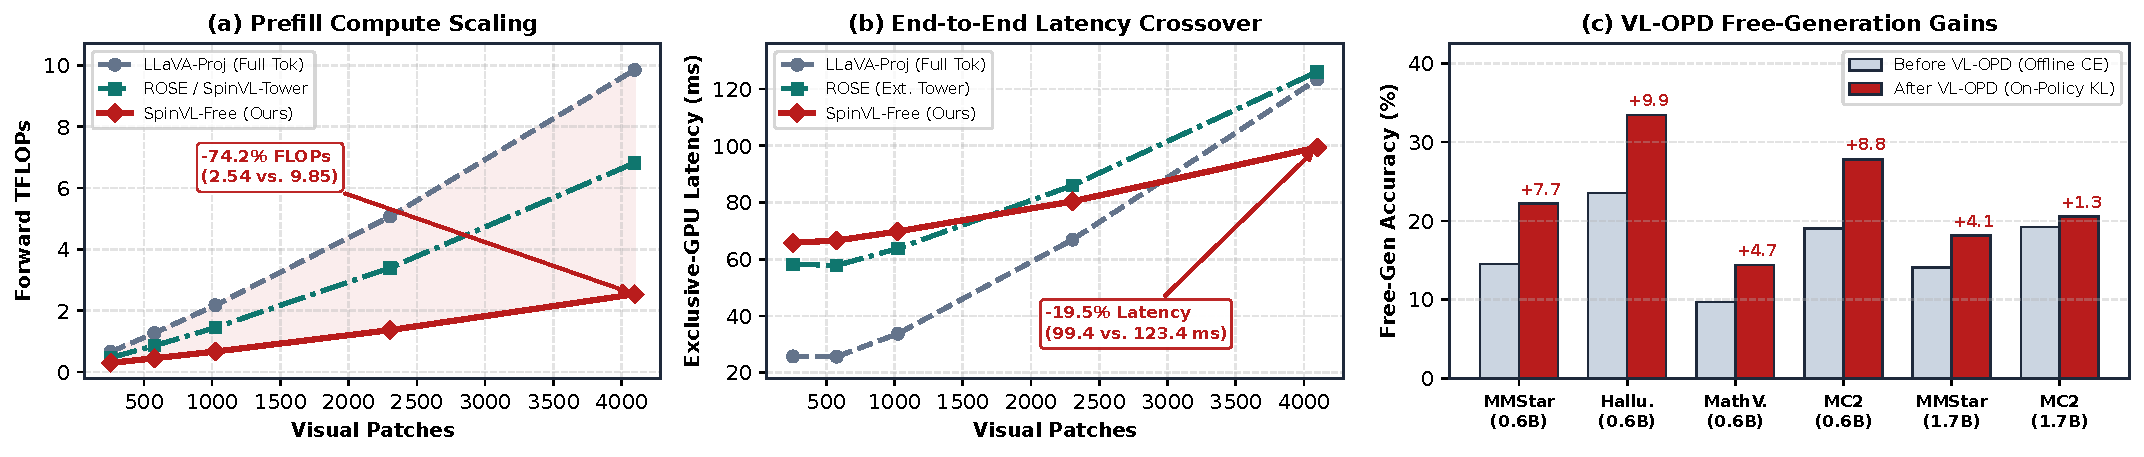
\includegraphics[width=0.95\textwidth]{fig_exp_highlights.pdf}
\caption{\textbf{High-resolution efficiency scaling and VL-OPD free-generation
gains.} \textbf{(a, b)} Prefill FLOPs and latency ($1.7$B, \texttt{hyb},
$T{=}64$; Tab.~\ref{tab:supp_eff}), achieving $-74.2\%$ FLOPs and $-19.5\%$
latency at $4{,}096$ patches. \textbf{(c)} Step~2 \texttt{VL-OPD} gains under
forced free-form greedy decoding ($0.6$B and $1.7$B, $28$k \emph{+open}).}
\label{fig:exp_highlights}
\end{figure*}

\subsection{Ablations}
\label{sec:abl}

\paragraph{Frontend parameterisation and depth.}
Tab.~\ref{tab:supp_front} and Fig.~\ref{fig:supp_abl}(a) isolate how to turn
the first $K{=}4$ frozen layers into a built-in encoder on $21$k \emph{base}
($s{=}0$). In \texttt{rel}, static rotation (\texttt{rot}) beats $201$M layer
copying ($40.73\%$ vs.\ $38.82\%$ MC2) and $K{=}0$ ($35.92\%$). In \texttt{ce}
with \texttt{mf} fixed, \texttt{rots} outperforms rank-$16$ LoRA by $+4.48$ MC2
($41.32\%$ vs.\ $36.84\%$) and larger grounding gap ($1.783$ vs.\ $1.667$) with
$36\%$ fewer parameters ($2.40$M vs.\ $3.74$M), and leads LoRA under
single-frequency rotation ($38.14\%$). Varying $K\in\{0,2,4,6\}$ on $28$k
\emph{+open} (Tab.~\ref{tab:supp_depth}, Fig.~\ref{fig:supp_abl}(b)) raises the
grounding gap from $0.387$ ($K{=}0$) to $0.896$ ($K{=}4$, $1.150$ three-seed
mean) and $0.978$ ($K{=}6$), lifting first-token accuracy from $30.7\%$ to
$36.0\%$--$38.0\%$ so $K{=}4$ provides the best compute--accuracy balance.

\paragraph{On-policy distillation and feature supervision.}
Tab.~\ref{tab:opd} and Fig.~\ref{fig:exp_highlights}(c) compare forward-KL
\texttt{VL-OPD} against GKD, MiniLLM, and SeqKD from the same $1.7$B
\emph{+open} checkpoint ($500$ steps). Although candidate scoring trails SeqKD
($40.35/32.90$ vs.\ $41.11/33.50$), forward KL keeps $95\%$ EOS termination
vs.\ $59\%$ for reverse KL (MiniLLM). Under forced free-form decoding,
\texttt{VL-OPD} lifts $0.6$B on MMStar ($+7.67$), HallusionBench ($+9.89$), and
MathVista ($+4.70$, $+8.78$ MC2), and raises $1.7$B on MMStar ($+4.06$),
MathVista ($+1.00$), and MC2 ($+1.30$; HallusionBench $-1.48$). Disabling
$\mathcal{L}_{\mathrm{feat}}$ (Sec.~\ref{sec:opd}) during joint training reaches
$42.63\%$ MC2 / $34.89\%$ Core3, showing end-to-end alignment suffices once
Stage~2 initializes RVE.

\begin{table}[t]
\centering
\caption{\textbf{Step~2 distillation objectives and free-generation gains}
($28$k \emph{+open}, $s{=}0$). Top: sequence/on-policy objectives from the same
$1.7$B \modelname-Free{} checkpoint ($500$ steps). Bottom: forced free-form
greedy generation without candidate scoring.}
\label{tab:opd}
\footnotesize
\setlength{\tabcolsep}{2.8pt}
\resizebox{\columnwidth}{!}{%
\begin{tabular}{@{}llcccc@{}}
\toprule
Objective / Pair & Split / Mode & Val CE$\downarrow$ & EOS$\uparrow$ & MC2$\uparrow$ & Core3$\uparrow$ \\
\midrule
Offline CE (Start)            & teacher-forced & 2.294 & 100.0\% & 41.09 & 33.76 \\
+ GKD~\citep{agarwal2024gkd}  & JSD ($\beta{=}0.5$) & 2.301 & \textbf{99.0\%} & 38.79 & 32.46 \\
+ MiniLLM~\citep{gu2024minillm} & Reverse KL   & 2.565 & 59.0\% & 40.46 & 32.34 \\
+ SeqKD~\citep{kim2016sequence} & Hard Top-$1$ & 2.417 & 84.0\% & \textbf{41.11} & \textbf{33.50} \\
+ VL-OPD (Ours)               & Forward KL      & 2.475 & 95.0\% & \underline{40.35} & \underline{32.90} \\
\midrule
\multicolumn{2}{@{}l}{\textit{Free-form greedy generation}} & MMStar & Hallu. & MathV. & MC2 \\
$0.6$B Free & before VL-OPD & 14.53 & 23.55 & 9.70 & 19.04 \\
            & after VL-OPD  & \textbf{22.20} & \textbf{33.44} & \textbf{14.40} & \textbf{27.82} \\
$1.7$B Free & before VL-OPD & 14.07 & 24.40 & 8.30 & 19.23 \\
            & after VL-OPD  & \textbf{18.13} & 22.92 & \textbf{9.30} & \textbf{20.53} \\
\bottomrule
\end{tabular}}
\end{table}

\subsection{Efficiency and Text Retention}
\label{sec:eff}

Fig.~\ref{fig:exp_highlights}(a,b) (full per-patch breakdown in
Tab.~\ref{tab:supp_eff}) quantifies resolution scaling. While LLaVA-Proj pays
$O((T{+}N)^2)$ across all $28$ layers, \modelname-Free{} confines $O(N^2)$ patch
attention to $K{=}4$ layers, crossing over in wall-clock time around ${\sim}3$k
patches and reaching $99.4$ vs.\ $123.4$\,ms ($19.5\%$ speedup) and $2.54$ vs.\
$9.85$ TFLOPs ($-74.2\%$) at $4{,}096$ patches. For text retention
(Fig.~\ref{fig:supp_mainres}(b)), bypassing RVE and SAVM preserves exact
unmodified backbone performance ($70.4\%$ GSM8K, $71.4\%$ ARC-C), whereas
permanently merging visual-only frontend adapters into layers $0$--$3$ without
text replay---as LoRA, pure rotation, or $W\mathrm{diag}(s)R_{\mathrm{s}}^{\top}$---drops
GSM8K to $0.0\%$, $0.0\%$, and $0.8\%$ (ARC-C to $27.4\%$, $24.2\%$, $23.4\%$).

\subsection{Boundary and Grounding Diagnostics}
\label{sec:boundary}

\begin{table}[t]
\centering
\caption{\textbf{Debiased $44$k mixture under unified frozen-backbone auditing}
($s{=}0$). Trained on the deduplicated, label-balanced $44$k split ($1{:}1$
Yes/No, $1{:}1{:}1{:}1$ A/B/C/D, zero shared test images) with unified greedy
decoding and relaxed ChartQA scoring. Full $3$-seed means and
\texttt{--force-gen} checks appear in Tab.~\ref{tab:supp_v6seeds}--Tab.~\ref{tab:supp_fgen}.}
\label{tab:grounding}
\footnotesize
\setlength{\tabcolsep}{1.8pt}
\resizebox{\columnwidth}{!}{%
\begin{tabular}{@{}lccccccccc@{}}
\toprule
Model ($44$k Debiased, $s{=}0$) & Val CE/EM & Gap$\uparrow$ & MMStar & Hallu. & MathV. & ChartQA & MC2 & Core3 & Avg6 \\
\midrule
LLaVA-Proj (Full Tok.)         & --- & --- & 28.60 & 52.05 & \textbf{25.70} & \textbf{10.52} & 40.33 & \textbf{35.45} & \textbf{20.77} \\
\midrule
ROSE (Single-Freq Rot.)        & 2.235/21.6\% & \textbf{1.345} & 26.07 & 48.16 & 18.40 & 0.72 & 37.11 & 30.88 & 15.70 \\
CA-Only ($R_{\ell}{\equiv}I$)  & 1.197/\textbf{41.2\%} & 0.187 & 28.27 & 52.16 & \textbf{23.90} & 9.44 & 40.21 & 34.77 & 19.59 \\
\textbf{\modelname-Tower (\texttt{srot}, $R_1$)} & 1.186/40.3\% & 0.239 & 28.20 & 53.21 & 23.30 & 9.04 & 40.70 & 34.90 & 19.63 \\
\textbf{\modelname-Tower (\texttt{mf}, $R_2$)}   & 1.189/40.5\% & 0.212 & \textbf{28.73} & \textbf{54.68} & 22.90 & 9.36 & \textbf{41.71} & \textbf{35.44} & \textbf{20.18} \\
\textbf{\modelname-Tower (\texttt{mf+qc}, $R_3$)} & \textbf{1.186}/39.5\% & 0.230 & 28.40 & 53.94 & 22.80 & \textbf{9.52} & 41.17 & 35.05 & 19.92 \\
\midrule
Patch-Merger ($K{=}0$, $S_0$)                    & 1.181/40.1\% & 0.068 & 27.67 & 52.16 & 22.90 & 9.44 & 39.91 & 34.24 & 19.58 \\
VoRA-style LoRA ($K{=}4$, $S_1$)                 & 1.163/40.3\% & 0.149 & 27.93 & 51.00 & 23.30 & 9.04 & 39.47 & 34.08 & 19.23 \\
\textbf{\modelname-Free (\texttt{rots}+CA, $F_2$)} & 1.835/26.4\% & 0.092 & 27.60 & \textbf{53.31} & 23.50 & 7.96 & 40.46 & 34.80 & 19.31 \\
\textbf{\modelname-Free (\texttt{rots}+\texttt{mf}, $S_2$)} & \textbf{1.155}/40.8\% & 0.152 & 28.87 & 49.42 & 23.60 & 9.44 & 39.14 & 33.96 & 19.29 \\
\textbf{+ Step 2 Cont.\ CE ($M_0$)}              & \textbf{1.155}/\textbf{41.2\%} & \textbf{0.192} & \textbf{29.40} & 52.47 & 23.50 & \textbf{9.88} & \textbf{40.94} & 35.12 & 19.99 \\
\textbf{+ Step 2 Off-Policy KD ($M_1$)}          & 1.229/39.9\% & 0.156 & 29.07 & \textbf{52.68} & 24.20 & 9.68 & 40.87 & \textbf{35.32} & \textbf{20.08} \\
\textbf{+ Step 2 Fwd-KL VL-OPD ($M_2$)}          & 1.233/40.8\% & 0.149 & 28.73 & 52.05 & \textbf{24.90} & 9.44 & 40.39 & 35.23 & 20.00 \\
\textbf{+ Step 2 JSD VL-OPD ($M_3$)}             & \textbf{1.154}/40.8\% & 0.181 & 28.60 & \textbf{52.68} & 23.50 & 9.64 & 40.64 & 34.93 & 19.85 \\
\bottomrule
\end{tabular}}
\end{table}

\paragraph{Format boundary and debiased $44$k auditing.}
Retraining on $28$k \emph{+open} doubles \modelname-Tower geometry accuracy
($1.83\%{\to}3.83\%$, Tab.~\ref{tab:supp_boundary}), whereas anchor-pooled
\texttt{hyb} leaves ChartQA near $1.2\%$; switching to \texttt{direct\_hyb} on
$44$k recovers ChartQA to $9.52\%$--$9.88\%$ ($94\%$ of LLaVA-Proj's $10.52\%$,
vs.\ $0.72\%$ ROSE), leaving dense OCR to hybrid sparse-token retention. On the
leakage-free, label-balanced $44$k audit (Tab.~\ref{tab:grounding}, full seeds
and \texttt{--force-gen} in Tab.~\ref{tab:supp_v6seeds}--Tab.~\ref{tab:supp_fgen}):
(1) Tangent bounding ($\tau_{\mathrm{rot}}{=}0.12$ on the five entry
projections) eliminates decoding collapse ($11.79\%{\to}40.89\%$--$41.33\%$ MC2,
$99.9\%$--$100.0\%$ EOS) and cuts full \texttt{qcond}+\texttt{direct\_hyb}
$4{,}096$-patch latency from $108.9$ to $101.9$\,ms ($19.9\%$ faster than
LLaVA-Proj's $127.2$\,ms, $2.67$ TFLOPs, $-72.5\%$); $3$-seed means rise
monotonically from $R_1$ to $R_3$ ($19.31\%{\to}19.52\%{\to}19.61\%$ Avg6,
$9.52\%$ ChartQA, $0.70\%$ OCRBench).
(2) Pairing RVE (\texttt{rots}, $K{=}4$) with bounded \texttt{mf} rotation
($S_2$) drops CE $1.835{\to}1.155$, lifts EM $26.4\%{\to}40.8\%$, and grows
grounding gap $2.24\times$ over $K{=}0$ ($0.152$ vs.\ $0.068$), outperforming
$K{=}4$ LoRA ($S_1$) on CE, EM, gap, and MMStar ($28.87\%$ vs.\ $27.93\%$).
(3) Step~2 over $S_2$ reaches $40.94\%$ MC2 / $35.32\%$ Core3 ($99.6\%$ of
LLaVA-Proj) via $M_0/M_1$, while \texttt{Fwd-KL VL-OPD} ($M_2$) achieves the
highest validation EM ($40.8\%$) and top tower-free MathVista ($24.90\%$),
showing competitive accuracy with zero deep visual tokens and an untouched LLM.
